Ein Superblock ist ein Stadtgebiet, welches für den Durchgangsverkehr (Autos und ÖV) gesperrt wird. Das Konzept stammt aus Barcelona und bezeichnet meistens einen 3$\times$3-Häuserblock, also ein Quartier aus 9 Häuserblocken, welches verkehrsberuhigt und begrünt wird (s. \cref{fig:superblocks}). Auch kleinere Formen, sogenannte \enquote{Miniblocks}, sind möglich.

\begin{figure}[H]
\centering
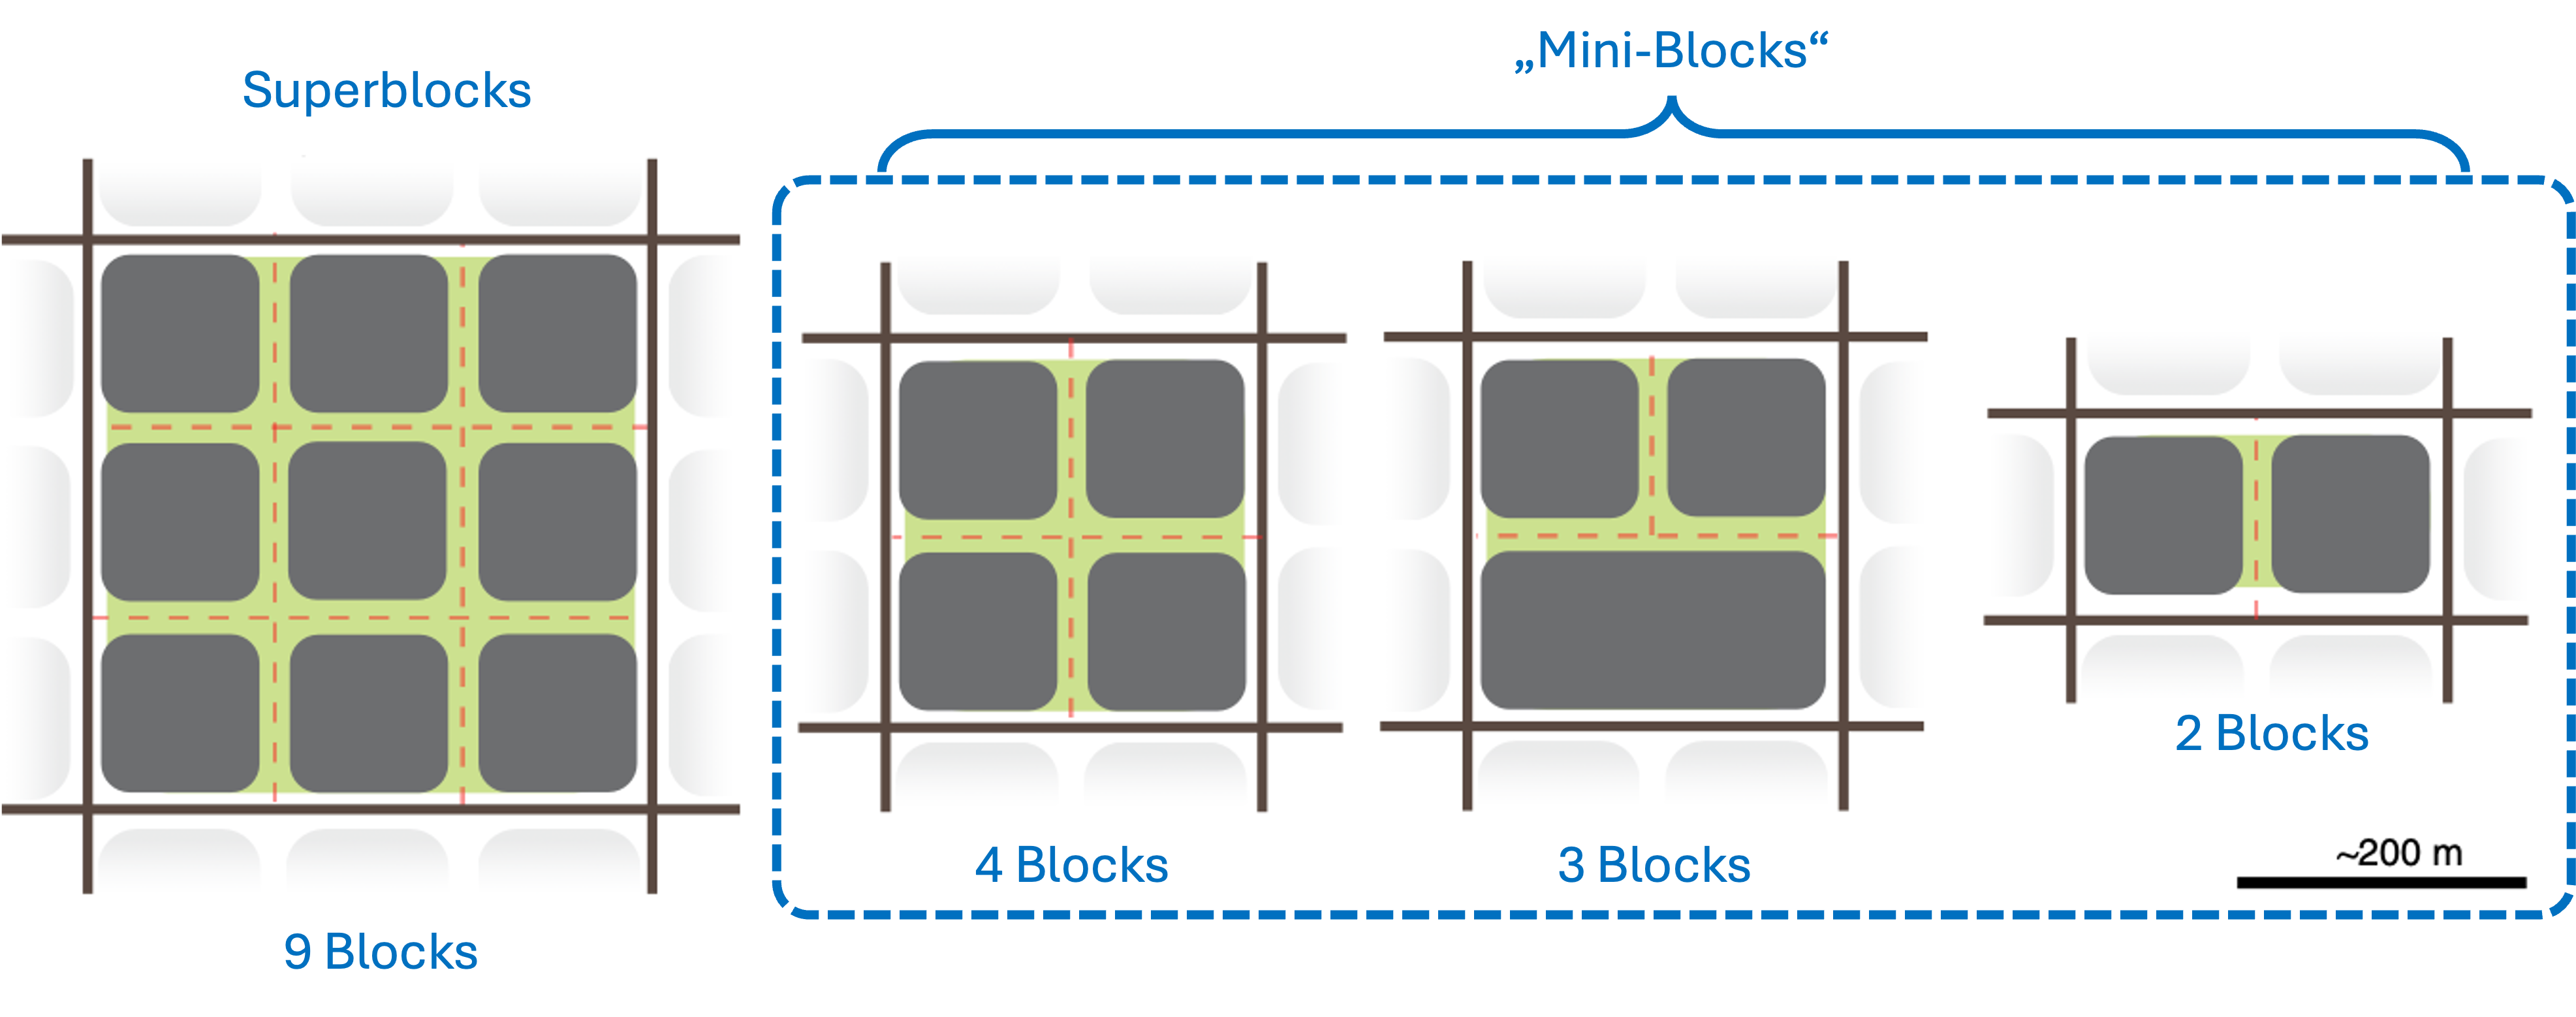
\includegraphics[width=0.7\linewidth]{Geografie/Stadtgeografie/Figures/Superblocks}
\caption{Superblocks, nach \cite{eggimannSchema}}
\label{fig:superblocks}
\end{figure}

Hauptmotivation für die Erstellung von Superblocks ist es, die Städte nachhaltiger, grüner und attraktiver für Bewohnerinnen sowie Touristen zu machen. Eine detailliertere Betrachtung der Vor- und Nachteile von Superblocks wird in \cref{subsec:beurteilen} erfolgen.

\section{Standorte für Superblocks bestimmen}
Um einen Superblock-Standort zu bestimmen, kommt es nicht nur auf die Form der Häuser darauf an, sondern auch auf andere Faktoren wie bespielsweise die Bevölkerungsdichte oder die Anzahl Fahrzeuge, welche täglich durch die Quartierstrassen fahren. Die Legende der Karte aus \cref{ex:superblock-zeichnen} ist in \cref{fig:legende} gezeigt.

\begin{figure}[H]
\centering
\includegraphics[width=.25\linewidth, page=1]{"Geografie/Stadtgeografie/Appendix/Karte Legende"}
\caption{Legende für die Karte aus \cref{ex:superblock-zeichnen}}
\label{fig:legende}
\end{figure}

Weitere Faktoren können für die Bestimmung geeigneter Superblock-Standorte relevant sein, beispielsweise:
\begin{enumerate}
\item Superblocks bringen weniger, wenn bereits viele Naherholungsgebiete in der Umgebung vorhanden sind
\item Superblocks sollten keine grossen Haupt-Verkehrsachsen blockieren, da es ansonsten zu Schleichverkehr durch Quartiere kommen kann.
\end{enumerate}

\begin{landscape}
\begin{myexercise}\label{ex:superblock-zeichnen}
Bestimmen Sie auf folgender Karte der Stadt Luzern einen möglichen Standort für einen Superblock. Mehrere Lösungen sind möglich! Berücksichtigen Sie dabei Bevölkerungsdichte und das Verkehrsaufkommen (s. Legende auf \cref{fig:legende}).

\begin{figure}[H]
\centering
\includegraphics[width=.95\linewidth, page=1]{"Geografie/Stadtgeografie/Appendix/Karte Luzern"}
\end{figure}
\begin{myanswer}
In einer Studie der ETH Zürich \cite{EGGIMANN2022106111}, bei der dieselben Faktoren beachtet und in wurden, wurden mittels einem mathematisch-räumlichen Modell folgende Gebiete als geeignete Superblock-Standorte hervorgehoben. Die dunklen Polygone sind traditionelle Superblock-Standorte, die hellen Polygone bezeichnen Standorte für mögliche Miniblocks.

\begin{figure}[H]
\centering
\includegraphics[width=0.5\linewidth]{"Geografie/Stadtgeografie/Appendix/Karte Luzern Sol"}
\caption{Geeignete Superblock-Gebiete nach \cite{EGGIMANN2022106111}}
\label{fig:karte-luzern-sol}
\end{figure}

Gut sichtbar ist, dass keine Hauptverkehrsachsen abgeschnitten werden und wenige Superblocks in Seenähe geplant werden (existierende Naherholungsgebiete). Ebenso ist eine rechteckige Form keine zwingende Voraussetzung für die Planung von Superblocks.
\end{myanswer}
\end{myexercise}
\end{landscape}

\section{Vor- und Nachteile von Superblocks beurteilen}
\label{subsec:beurteilen}
Lesen Sie die folgenden Pro- und Kontra-Artikel, und heben Sie die Hauptargumente hervor.
\newpage
\begin{tcolorbox}[title=Kontra-Argumente,
			parbox=false,
			colback=Crimson!10,
			colframe=Crimson,
			colbacktitle=Crimson]
\section*{Superblocks: Der urbane Albtraum im grünen Gewand}
Superblocks werden als revolutionäres Stadtplanungskonzept gefeiert. Sie sollen Verkehr reduzieren, Quartiere aufwerten und die Lebensqualität steigern. Doch was passiert wirklich? Wer profitiert, wer verliert – und welchen Preis zahlen wir alle?

\subsection*{Ausweichverkehr: Mehr Stau, weniger Mobilität}

Innerhalb der Superblocks herrscht Ruhe, doch der Verkehr verlagert sich auf umliegende Wohnquartiere. Anwohner der Umgebung leiden unter Ausweichverkehr, längeren Wegen und verstopften Strassen. Der Verkehr verschwindet nicht – er sucht sich neue, oft schlechtere Wege. Lebenswichtiger Verkehr wie Polizei, Feuerwehr und Krankenwagen werden durch die Einschränkungen gehindert und verlangsamt.

\subsection*{Gated Communities 2.0 – Gentrifizierung unter neuem Namen}
Superblocks treiben die Mieten in die Höhe und verdrängen Alteingesessene, während Wohlhabende die autofreien Zonen geniessen. Investoren wittern Chancen, Luxuswohnungen ersetzen günstigen Wohnraum, und die soziale Durchmischung weicht exklusiven Quartieren. Wer nicht mithalten kann, wird an den Stadtrand gedrängt, während sich innerhalb der Superblocks eine abgeschottete Wohlstandselite etabliert. Was als soziale Verbesserung verkauft wird, ist in Wahrheit nichts anderes als Gentrifizierung im grünen Gewand.

\subsection*{Wirtschaftlicher Niedergang}
Eingeschränkte Zufahrtsmöglichkeiten machen es lokalen Gewerben schwer. Lieferanten kämpfen mit Umwegen, Kunden bleiben aus, und viele Betriebe müssen schliessen. Der einst belebte Stadtteil verliert an wirtschaftlicher Dynamik, die Steuereinnahmen sinken, und statt florierender Viertel bleiben sterile Wohnzonen ohne funktionierendes Gewerbe zurück.

\subsection*{Strassen sind keine Parks}
Superblocks suggerieren, dass Strassen als lebenswerte Räume ausreichen, doch das ist eine Fehlplanung. Asphalt mit Sitzbänken ersetzt keine echten Parks mit grossen Grünflächen, Wasser, Bäumen und natürlicher Vielfalt. Statt halbgare ``Begegnungszonen'' zu schaffen, sollte Stadtentwicklung echte Erholungsräume schaffen.

\subsection*{Sicherheit in den Superblocks – Verwahrlosung statt urbaner Idylle}
Die versprochenen Freiräume der Superblocks verkommen oft zu unsicheren Zonen. Statt lebendiger Begegnungsorte entstehen Rückzugsräume für Herumlungernde, begleitet von Alkohol, weggeworfenen Spritzen und mangelnder sozialer Kontrolle. Was als offene, sichere Stadt geplant war, entwickelt sich zu einem Brennpunkt für Verwahrlosung und Kriminalität.

\subsection*{Fazit: Eine urbane Fehlkonstruktion}

Superblocks lösen keine Probleme, sie verlagern sie. Sie bringen mehr Stau, höhere Mieten und eine Entfremdung zwischen Stadtbewohnern. Wer glaubt, dass Poller und autofreie Strassen die Stadt der Zukunft sind, ignoriert die langfristigen Folgen. Superblocks sind kein Fortschritt – sie sind ein Rückschritt in grüner Verpackung.


\end{tcolorbox}
\newpage
\begin{tcolorbox}[title=Pro-Argumente,
			parbox=false,
			colback=ForestGreen!10,
			colframe=ForestGreen,
			colbacktitle=ForestGreen]
\section*{Superblocks: Die Zukunft lebenswerter Städte}

Superblocks haben das Potenzial, Städte lebenswerter zu machen. Sie reduzieren den Autoverkehr, schaffen mehr Raum für Menschen und fördern soziale Gerechtigkeit. Doch warum ist dieses Konzept so vielversprechend?

\subsection*{Mehr Raum für Menschen, weniger für Autos}
Superblocks verringern die Dominanz des Autos in Innenstädten. Ruhige, verkehrsberuhigte Quartiere verbessern Luftqualität und Lärmschutz, während Fussgänger und Radfahrer profitieren. Strassen werden sicherer, so dass Kinder gefahrlos spielen und sich Menschen frei bewegen können. Autofahren wird weniger attraktiv, so dass auch in der gesamten Stadt weniger gefahren wird.


\subsection*{Soziale Vorteile: Mehr Begegnungen, stärkere Gemeinschaft}
Superblocks fördern das Miteinander, indem sie öffentlichen Raum neu gestalten. Weniger Verkehr bedeutet mehr Begegnungsmöglichkeiten, wodurch Nachbarschaften gestärkt werden. Plätze und Strassen werden wieder zu lebendigen Treffpunkten für alle Generationen.

\subsection*{Gesunde Städte fördern gesunde Menschen}
Weniger verschmutzte Städte führen zu weniger Atemwegserkrankungen und retten Leben. Nebst physischen Vorteilen entstehen jedoch auch psychische Vorteile durch Stressreduktion sowie vermehrte soziale Interaktionen. 

\subsection*{Wirtschaftlicher Aufschwung für lokale Betriebe}
Fussgängerfreundliche Städte bringen wirtschaftliche Vorteile: Cafés, Boutiquen und kleine Geschäfte profitieren von mehr Laufkundschaft. Erfahrungen aus Barcelona zeigen, dass Superblocks lokale Unternehmen stärken statt schwächen.

\subsection*{Nachhaltigkeit: Städte klimafreundlich gestalten}
Superblocks reduzieren den Autoverkehr erheblich und senken damit CO$_2$-Emissionen. Gleichzeitig schaffen zusätzliche Grünflächen ein angenehmeres Stadtklima. Durch bessere Infrastruktur für Fahrräder und öffentliche Verkehrsmittel wird umweltfreundliche Mobilität gefördert.

\subsection*{Kostengünstige und flexible Umsetzung}
Im Gegensatz zu teuren Bauprojekten lassen sich Superblocks mit günstigen und einfachen Massnahmen wie Pollern und Begrünung umsetzen. Sie senken langfristig Kosten durch weniger Verkehrsunfälle und geringere Gesundheitsbelastungen. Zudem lässt sich die Lösung in fast allen Städten umsetzen -- auch in Städten ohne Schachbrettmuster.

\subsection*{Fazit: Städte für Menschen statt für Autos gestalten}
Superblocks sind eine bewährte Lösung für moderne Stadtentwicklung. Sie schaffen nachhaltige, soziale, gesundheitliche und wirtschaftliche Vorteile, indem sie den öffentlichen Raum neu denken – als Orte des Zusammenlebens, der Erholung und der urbanen Kultur.

\end{tcolorbox}
\newpage

\begin{myexercise}
Notieren Sie sich während dem Anschauen des \href{https://www.srf.ch/play/tv/10-vor-10/video/superblocks---stadtstrassen-begruenen-statt-befahren?urn=urn:srf:video:2edec553-2a82-435c-92a5-824bd5312f04}{10-vor-10-Videos über Superblocks} die genannten Vor- und Nachteile von Superblocks.

\begin{table}[H]
\centering
\begin{tabular}{p{.45\textwidth}|p{.45\textwidth}}
\textbf{Vorteile} & \textbf{Nachteile} \\\midrule\midrule
&\\[300 pt]
\end{tabular}
\end{table}
\begin{myanswer}
\begin{table}[H]
\centering
\begin{tabular}{p{.45\textwidth}|p{.45\textwidth}}
\textbf{Vorteile} & \textbf{Nachteile} \\\midrule\midrule
Grünere Städte (Gesundheit, Wohlbefinden und Ästhetik) & Partys und Lautstärke in der Nacht, Littering\\\midrule
Platz für FussgängerInnen und Velos (statt Autos)& Zunahme des Verkehrs rund um Superblocks\\\midrule
Mehr Begegnungsmöglichkeiten&Verteuerung der Mieten\\\midrule
Vorteile für das Klima und Luftqualität & Parkplätze aufgehoben\\\midrule
Anstieg der Kundschaft in Geschäften &\\
\end{tabular}
\end{table}

Weitere, im Video nicht explizit genannte Aspekte aus der Podiumsdiskussion: 
\begin{enumerate}
\item \textbf{Pro-Seite}: Nachhaltigkeit und CO$_2$-Reduktion der Städte
\item \textbf{Kontra-Seite}: Strassen sind keine Parks, mögliche negative Aspekte auf die Wirtschaft
\end{enumerate}
\end{myanswer}
\end{myexercise}
\newpage

\begin{mychallenge}\label{ex:superblock-zeichnen-sursee}
Würde die Erstellung von Superblocks auch in einer Stadt wie Sursee Sinn ergeben? Argumentieren Sie, indem Sie folgende Karte verwenden. Erklären Sie zudem, ob die Vor- und Nachteile aus \cref{subsec:beurteilen} für die Stadt Sursee ebenso gelten. Die Legende zur Karte ist in \cref{fig:legende} abgebildet.

\begin{figure}[H]
\centering
\includegraphics[width=.8\linewidth, page=1]{"Geografie/Stadtgeografie/Appendix/Karte Sursee"}
\end{figure}

\begin{myanswer}
Einige Ansätze für die Antwort:

Da das Verkehrsaufkommen geringer ist und viele Naherholungsgebiete vorhanden sind (See, Hügel, Parks, etc.), scheint das Problem weniger dringlich, die positiven Nutzen sind also insgesamt geringer, währenddem die Gefahren für das Gewerbe ähnlich hoch an anderen Orten sind. Sicherheitsbedenken und Gefahren für Gentrifikation sollten aufgrund der Kleinräumigkeit von Sursee eine untergeordnete Rolle spielen. Im Zentrum der Stadt Sursee wären Miniblocks oder Superblocks aber durchaus denkbar.

\end{myanswer}
\end{mychallenge}

\begin{mychallenge}[Vertiefungsartikel zu Superblocks]
\begin{figure}[H]
\centering
\colorbox{white}{\includegraphics[width=.8\linewidth]{"Geografie/Stadtgeografie/Appendix/2024-07-16 NZZ Superblocks"}}
\end{figure}
\end{mychallenge}


\section{Lernziele}

\begin{todolist}
\item Ich kann benennen und grafisch darstellen, welche städteplanerischen Massnahmen mit dem Konzept ``Superblocks'' verbunden sind.
\item Ich kann Datenmaterial eines Stadtquartiers interpretieren (Stadtkarten, Bevölkerungsdichte, Verkehrsaufkommen) und erörtern, inwiefern sich dieses Stadtquartier für Superblocks eignet oder nicht.
\item Ich kann beurteilen und begründen, welche Vor- und Nachteile Superblocks in den Dimensionen Umwelt, Soziales, Wirtschaft und Sicherheit mit sich bringen.
\item Ich kann basierend auf verschiedenen Perspektiven zum Thema ``Superblocks'' mein eigenes Urteil bilden.
\end{todolist}